\documentclass{beamer}
\usetheme{zgca}
\usepackage{tikz}
\usepackage{wrapfig}
\usepackage{booktabs}

% Set the background image for the title slide
\titlebackground{assets/background}

\title{OPD Interpretability and Better Recipe}
\subtitle{关于On-Policy一些分析性工作的分享}
\author{林佳豪}
\date{2026.6.12}

\begin{document}

% Slide 1: Cover Page (Using standard template maketitle)
\maketitle

% Define Section with Paper Title
\section{Rethinking On-Policy Distillation of Large Language Models}

% Slide 2: 本文观察的对齐指标
\begin{frame}[t]{本文观察的对齐指标}
  \small
  设学生 top-$k$ 集合为 $S_t^{(p)}$，教师为 $S_t^{(q)}$。

  \vspace{0.1cm}
  \textbf{Overlap Ratio}：师生 top-$k$ 集合的重合比例。
  \[
    \mathcal{M}_{\text{overlap}} \triangleq \mathbb{E}_{t} \left[ \frac{|S_t^{(p)} \cap S_t^{(q)}|}{k} \right]
  \]

  \textbf{Overlap-Token Advantage}：重合 Token 上学生与教师归一化概率的加权差异，趋于 $0$ 表示对齐。
  \[
    \mathcal{M}_{\text{adv}} \triangleq \mathbb{E}_{t}\!\left[ \frac{1}{|S_t^{(p)} \cap S_t^{(q)}|} \sum_{v \in S_t^{(p)} \cap S_t^{(q)}} \bar{p}_t(v) \bigl(\log \bar{q}_t(v) - \log \bar{p}_t(v)\bigr) \right]
  \]

  \textbf{Entropy Gap}：师生在学生生成轨迹上的熵差，收敛至 $0$ 表示置信度分布匹配。
  \[
    \Delta H_t = \left| H(q_t) - H(p_t) \right|
  \]
\end{frame}

% Slide 3: 现象1.1：初始匹配度判据 (实验设置与教师性能)
\begin{frame}[t]{\underline{现象1.1：} 初始匹配度 (实验设置)}
  \begin{columns}[T,onlytextwidth]
    \begin{column}{0.48\textwidth}
      \small
      \textbf{实验设置}：
      \begin{itemize}
        \item \textbf{学生模型}：Qwen3-1.7B-Base
        \item \textbf{教师模型}：
          \begin{itemize}
            \item Qwen3-4B-Base-GRPO (同系列RL)
            \item Qwen3-4B (不同系列)
          \end{itemize}
      \end{itemize}
      \vspace{0.1cm}
      \textbf{初始教师性能}：Qwen3-4B-Base-GRPO是Qwen3-4B-Base经过GRPO训练1 Epoch得到的思考模型，其 Benchmark 性能与常规非思考教师相当。
    \end{column}
    \begin{column}{0.48\textwidth}
      \centering
      \includegraphics[width=\linewidth,height=3.8cm,keepaspectratio]{references/Rethinking On-Policy Distillation of Large Language Models Phenomenology, Mechanism, and Recipe/Figures/4.1/tch_val/5_1_teacher_perf.pdf}
    \end{column}
  \end{columns}
  \vspace{0.5cm}
  \footnotesize
  全文OPD数据集\textbf{皆为DAPO-Math-17K}，后续不再重复标注。
\end{frame}

% Slide 3: 现象1.2：初始匹配度判据 (蒸馏结果与结论)
\begin{frame}[t]{\underline{现象1.2：} 初始匹配度 (结果与结论)}
  \begin{center}
    \includegraphics[width=\textwidth,height=3.8cm,keepaspectratio]{references/Rethinking On-Policy Distillation of Large Language Models Phenomenology, Mechanism, and Recipe/Figures/3.1/3_1_metrics.pdf}
  \end{center}
  
  \textbf{实验结果}：
  \begin{itemize}
    \item Qwen3-4B-Base-GRPO的蒸馏效果显著更好；
    \item 学生与Qwen3-4B-Base-GRPO的分布一致性比Qwen3-4B更高。
  \end{itemize}
\end{frame}

% Slide 4: 现象2.1：新输出模式的作用 (实验设置)
\begin{frame}[t]{\underline{现象2.1：} 新输出模式的作用 (实验设置)}
  \textbf{实验设置}：\par
  为了验证“新输出模式”对 OPD 蒸馏的影响，本实验在 DeepSeek-Distill 和 Qwen 两个模型家族上，分别对比了使用\textbf{RL后教师}与\textbf{无RL教师}进行蒸馏的效果。

  \begin{itemize}
    \item \textbf{DeepSeek-Distill 家族实验设置}：
      \begin{itemize}
        \item 学生模型：DeepSeek-R1-Distill-Qwen-1.5B
        \item 教师模型：Skywork-OR1-Math-7B \slash R1-Distill-7B
      \end{itemize}
    \item \textbf{Qwen 家族实验设置}：
      \begin{itemize}
        \item 学生模型：Qwen3-1.7B (Non-thinking)
        \item 教师模型：Qwen3-4B-Non-Thinking-RL-Math\slash Qwen3-4B
      \end{itemize}
  \end{itemize}
\end{frame}

% Slide 5: 现象2.2：新输出模式的作用 (结果与结论)
\begin{frame}[t]{\underline{现象2.2：} 新输出模式的作用 (结果与结论)}
  \noindent\makebox[\textwidth][c]{%
    \includegraphics[width=0.4\linewidth]{references/Rethinking On-Policy Distillation of Large Language Models Phenomenology, Mechanism, and Recipe/Figures/3.2/DS/Figure5A.pdf}%
    \includegraphics[width=0.4\linewidth]{references/Rethinking On-Policy Distillation of Large Language Models Phenomenology, Mechanism, and Recipe/Figures/3.2/Qwen/Figure5B.pdf}%
  }\par

  \vspace{0.1cm}
  \textbf{实验结果}：纯靠规模变大的常规教师对学生提升非常有限；而经历额外 RL形成新输出模式的教师能为学生带来显著的性能增益。
\end{frame}

% Slide 6: 现象3：逆向蒸馏
\begin{frame}[t]{\underline{现象3：} 逆向蒸馏}
  \begin{columns}[T,onlytextwidth]
    \begin{column}{0.3\textwidth}
      \textbf{实验设置}：
      \begin{itemize}
        \item 学生：JustRL-DeepSeek-1.5B
        \item 教师：
        \begin{itemize}
          \item R1-Distill-1.5B
          \item R1-Distill-7B
        \end{itemize}
      \end{itemize}
    \end{column}
    \begin{column}{0.7\textwidth}
      \centering
      \includegraphics[width=\linewidth,height=4.5cm,keepaspectratio]{references/Rethinking On-Policy Distillation of Large Language Models Phenomenology, Mechanism, and Recipe/Figures/3.2/JustRL/JustRL_val.pdf}
    \end{column}
  \end{columns}

  \vspace{0.1cm}
  \textbf{结果}：
  \begin{itemize}
    \item 从无RL同规模教师蒸馏时，学生退回无 RL 水平；
    \item 增大无RL教师的规模，退化轨迹和结果几乎一致。
  \end{itemize}
  \textbf{主要结论}：教师规模和分数不能决定OPD效果。
\end{frame}

% Slide 7: 分析1.1：渐进对齐 (实验设置)
\begin{frame}[t]{\underline{分析1.1：} 追踪token重叠率 (实验设置)}
  \begin{columns}[T,onlytextwidth]
    \begin{column}{0.3\textwidth}
      \textbf{实验设置}：
      \begin{itemize}
        \item 学生：R1-Distill-1.5B
        \item 教师：
        \begin{itemize}
          \item JustRL-1.5B (经 RL)
          \item R1-Distill-7B (无 RL)
        \end{itemize}
      \end{itemize}
    \end{column}
    \begin{column}{0.68\textwidth}
      \centering
      \includegraphics[width=\linewidth,height=4.5cm,keepaspectratio]{references/Rethinking On-Policy Distillation of Large Language Models Phenomenology, Mechanism, and Recipe/Figures/5.1/5_1_combined.pdf}
    \end{column}
  \end{columns}

  \vspace{0.1cm}
  两者 Benchmark 性能相当（7B 略高），但蒸馏结果截然不同。\par
  JustRL-1.5B恢复了 $80\%$+ 的师生性能差距；R1-Distill-7B无任何提升。
\end{frame}

% Slide 8: 分析1.2：渐进对齐 (动力学)
\begin{frame}[t]{\underline{分析1.2：} 追踪token重叠率 (结果)}
  \begin{columns}[T,onlytextwidth]
    \begin{column}{0.3\textwidth}
      \textbf{三个对齐指标的动态对比}：
      \begin{itemize}
        \item \textbf{Overlap Ratio}：成功设置从 $72\%$ 稳步升至 $91\%$ 以上，失败设置停滞。
        \item \textbf{Overlap-Token Advantage}：成功设置趋向 $0$，失败设置无变化。
      \end{itemize}
    \end{column}
    \begin{column}{0.68\textwidth}
      \centering
      \includegraphics[width=\linewidth,height=4.5cm,keepaspectratio]{references/Rethinking On-Policy Distillation of Large Language Models Phenomenology, Mechanism, and Recipe/Figures/5.1/5_1_combined.pdf}
    \end{column}
  \end{columns}

  \begin{itemize}
    \item \textbf{Entropy Gap}：成功设置收敛（学生置信度分布趋近教师），失败设置不收敛。
  \end{itemize}
\end{frame}

% Slide 9: 分析2：仅优化共享 Token 便足够
\begin{frame}[t]{\underline{分析2：} 仅优化重叠Token}
  \begin{columns}[T,onlytextwidth]
    \begin{column}{0.3\textwidth}
      \textbf{实验设置}：
      \begin{itemize}
        \item 学生：R1-Distill-1.5B
        \item 教师：JustRL-1.5B
      \end{itemize}
      \textbf{消融变体}：
      \begin{itemize}
        \item Student Top-$k$：优化全支持域
        \item Overlap Top-$k$：只优化交集
        \item Non-Overlap Top-$k$：只优化差集
      \end{itemize}
    \end{column}
    \begin{column}{0.7\textwidth}
      \centering
      \includegraphics[width=\linewidth,height=4.5cm,keepaspectratio]{references/Rethinking On-Policy Distillation of Large Language Models Phenomenology, Mechanism, and Recipe/Figures/5.2/5_2_combined.pdf}\par
      \textbf{主要结论}：仅优化 Overlap Top-$k$ 即可匹配 Student Top-$k$ 的全部增益，非重合部分几乎无贡献。
    \end{column}
  \end{columns}
\end{frame}

% Slide 10: 配方1：教师 Rollout 离策冷启动
\begin{frame}[t]{\underline{配方1：} 学生SFT冷启动}
  \textbf{动机}：师生分布差异大时直接 OPD 效果差，先 SFT 拉近距离。
  \begin{columns}[T,onlytextwidth]
    \begin{column}{0.3\textwidth}
      \footnotesize
      \textbf{实验设置}：（同现象1）
      \begin{itemize}
        \item 学生：Qwen3-1.7B-Base
        \item 教师：Qwen3-4B (Non-thinking)
      \end{itemize}
      \textbf{两阶段训练}：
      \begin{itemize}
        \item SFT：用教师在OpenThoughts3生成的200K数据微调学生
        \item OPD
      \end{itemize}
    \end{column}
    \begin{column}{0.68\textwidth}
      \centering
      \includegraphics[width=\linewidth,height=4.2cm,keepaspectratio]{references/Rethinking On-Policy Distillation of Large Language Models Phenomenology, Mechanism, and Recipe/Figures/4.2/4_2_combined.pdf}
    \end{column}
  \end{columns}

  \vspace{0.1cm}
  \textbf{结果}：SFT 冷启动显著拉高初始 Overlap、降低熵差，提升后续 OPD 最终性能上限。
\end{frame}

% Slide 11: 配方2.1：对齐后训练提示词 (模板对齐)
\begin{frame}[t]{\underline{配方2：} 对齐教师后训练模板}
  \textbf{动机}：教师策略由后训练时见过的提示词塑造，匹配其模板可提升分布兼容性。
  \begin{columns}[T,onlytextwidth]
    \begin{column}{0.3\textwidth}
      \footnotesize
      \textbf{实验设置}：
      \begin{itemize}
        \item 学生：R1-Distill-1.5B
        \item 教师：JustRL-1.5B
      \end{itemize}
      \textbf{模板对比}（同为DAPO-Math-17K）：
      \begin{itemize}
        \item DAPO格式（数据集原格式）
        \item 统一\texttt{boxed}格式（教师后训练数据格式）
      \end{itemize}
    \end{column}
    \begin{column}{0.68\textwidth}
      \centering
      \includegraphics[width=\linewidth,height=4.5cm,keepaspectratio]{references/Rethinking On-Policy Distillation of Large Language Models Phenomenology, Mechanism, and Recipe/Figures/4.3/4_3_Same.pdf}
    \end{column}
  \end{columns}

  \vspace{0.1cm}
  \textbf{结果}：仅切换模板即带来更高的 Overlap 增长和准确率提升，模板一致性在 Token 级别强烈影响分布兼容性。
\end{frame}

% Slide 12: 配方2.2：对齐后训练提示词 (内容与混合)
\begin{frame}[t]{\underline{配方3：} 对齐教师后训练题目}
  \textbf{动机}：使用教师后训练时的相同数据集，可以让教师发挥最大能力。

  \begin{columns}[T,onlytextwidth]
    \begin{column}{0.3\textwidth}
      \footnotesize
      \textbf{实验设置}：
      \begin{itemize}
        \item 学生：Qwen3-1.7B-Base
        \item 教师：Qwen3-4B-Base-GRPO
      \end{itemize}
      \textbf{训练数据对比}：
      \begin{itemize}
        \item DAPO-Math-17K（教师 RL 数据集）
        \item DeepMath 子集（同领域 OOD 数据集）
      \end{itemize}
    \end{column}
    \begin{column}{0.68\textwidth}
      \centering
      \includegraphics[width=\linewidth,height=4.5cm,keepaspectratio]{references/Rethinking On-Policy Distillation of Large Language Models Phenomenology, Mechanism, and Recipe/Figures/4.3/4_3_Diff.pdf}
    \end{column}
  \end{columns}

  \vspace{0.1cm}
  \textbf{结果}：教师在后训练过的数据集上教学，能与学生有\textbf{更多重叠token}，但仅用这些数据会导致\textbf{熵过度降低}。
\end{frame}

% Slide 13: 讨论1：响应长度存在最佳区间
\begin{frame}[t]{\underline{讨论1：} 响应长度的最佳区间}
  \textbf{问题}：教师的 token 级奖励在学生生成的前缀上计算，前缀越长漂移越大，奖励质量会下降？
  \begin{columns}[T,onlytextwidth]
    \begin{column}{0.25\textwidth}
      \textbf{实验设置}：
      \begin{itemize}
        \item 学生：R1-Distill-1.5B
        \item 教师：JustRL-1.5B
      \end{itemize}
      \textbf{变量}：最大响应长度 0.5K--15K
    \end{column}
    \begin{column}{0.74\textwidth}
      \centering
      \includegraphics[width=\linewidth,height=4.2cm,keepaspectratio]{references/Rethinking On-Policy Distillation of Large Language Models Phenomenology, Mechanism, and Recipe/Figures/6.1.2/6_1_response_summary.pdf}
    \end{column}
  \end{columns}

  \vspace{0.1cm}
  \textbf{关键发现}：3K--7K 最佳；教师相对于学生的优势随前缀长度单调下降。
\end{frame}

% Slide 14: 讨论2：Sampled-Token Reward 已足够
\begin{frame}[t]{\underline{讨论2：} Top-K的超参K选择}
  \textbf{问题}：Top-$k$ OPD 需要选择支撑集大小 $k$，这个超参数如何选择？\par
  \textbf{实验设置}：
  \begin{itemize}
    \item 学生 R1-Distill-1.5B，教师 JustRL-1.5B
    \item 对比： Sampled-Token 与 Top-$k$ ($k{=}1,4,16,64$)
  \end{itemize}

  \begin{columns}[T,onlytextwidth]
    \begin{column}{0.42\textwidth}
      \centering
      \includegraphics[width=\linewidth,height=3.5cm,keepaspectratio]{references/Rethinking On-Policy Distillation of Large Language Models Phenomenology, Mechanism, and Recipe/Figures/6.2/5_1_effect_of_k_topk.pdf}
    \end{column}
    \begin{column}{0.56\textwidth}
      \centering
      \includegraphics[width=\linewidth,height=3.5cm,keepaspectratio]{references/Rethinking On-Policy Distillation of Large Language Models Phenomenology, Mechanism, and Recipe/Figures/6.2/6_2_combined.pdf}
    \end{column}
  \end{columns}

  \vspace{0.1cm}
  \textbf{关键发现}：$k{\ge}4$ 与 Sampled-Token 性能相当，Top-1 因 mode-concentrated 选择规则导致不稳定。OPD 的 $k$ 不是关键超参，避免退化的 Top-1 即可。
\end{frame}

% Slide 16: 总结
\begin{frame}[t]{总结}
  \begin{columns}[T,onlytextwidth]
    \begin{column}{0.48\textwidth}
      \textbf{OPD 何时有效？}
      \begin{itemize}
        \item 师生需要是同一系列模型；
        \item 教师需具备学生尚未拥有的新输出模式，不仅是分数更高；
        \item 响应长度在最佳区间（3K--7K）。
      \end{itemize}
    \end{column}
    \begin{column}{0.48\textwidth}
      \textbf{最佳 Recipe}
      \begin{itemize}
        \item 用教师生成的 Rollout 对学生做 SFT 冷启动，拉高初始 Overlap。
        \item 对齐教师后训练时的提示词模板，提升分布兼容性；
        \item 使用教师后训练数据，但需混合 OOD 数据以防熵坍塌；
        \item Sampled-Token 或 Top-$k$ ($k{\ge}4$)。
      \end{itemize}
    \end{column}
  \end{columns}
\end{frame}


% Define Section with Paper Title
\section{Revisiting On-Policy Distillation}

% Slide 17: 理论分析1.1：偏差-方差权衡（推导）
\begin{frame}[t]{\underline{问题1.1}：偏差-方差权衡（理论分析）}
  定义 $r_t = \log \frac{\pi_\theta(y_t \mid c_t)}{q(y_t \mid c_t)}$，$s_t = \nabla_\theta \log \pi_\theta(y_t \mid c_t)$。

  \begin{columns}[T,onlytextwidth]
    \small
    \begin{column}{0.48\textwidth}
      \textbf{序列级 OPD}（$\gamma{=}1$）：
      \[
        \hat{g}_{\mathrm{seq}} = \sum_{t=1}^{T} \left(\sum_{t'=t}^{T} r_{t'}\right) s_t
      \]
      无偏，慢，worst-case 方差 $\mathcal{O}(T^4)$。
    \end{column}
    \begin{column}{0.48\textwidth}
      \textbf{Token 级 OPD}（$\gamma{=}0$，有偏）：
      \[
        \hat{g}_{\mathrm{tok}} = \sum_{t=1}^{T} r_t \, s_t
      \]
      有偏，快，worst-case 方差 $\mathcal{O}(T^2)$。
    \end{column}
  \end{columns}

  \vspace{0.1cm}
  \textbf{$\gamma$-插值}（$\gamma \in [0,1]$）：
  \[
    \hat{g}_{\gamma} = \sum_{t=1}^{T} \left(\sum_{t'=t}^{T} \gamma^{t'-t} r_{t'}\right) s_t
  \]
  \textbf{核心权衡}：序列级无偏但方差随序列长度\textbf{四次增长}，Token 级有偏但方差仅\textbf{二次增长}。
\end{frame}

% Slide 18: 理论分析1.2：偏差-方差权衡（玩具实验）
\begin{frame}[t]{\underline{问题1.2}：偏差-方差权衡（玩具实验）}
  \begin{columns}[T,onlytextwidth]
    \begin{column}{0.52\textwidth}
      \centering
      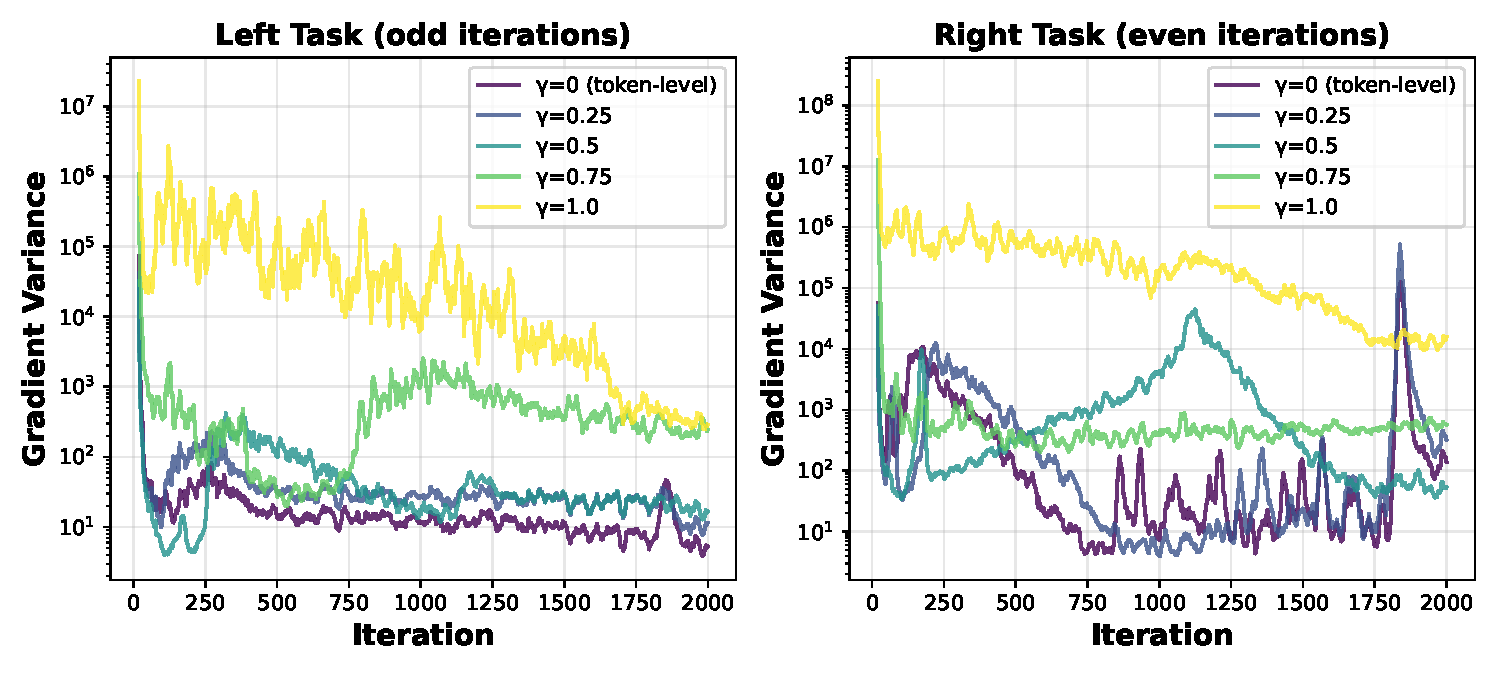
\includegraphics[width=\linewidth,height=4cm,keepaspectratio]{references/Revisiting On-Policy Distillation Empirical Failure Modes and Simple Fixes/figures/toy_variance.pdf}
    \end{column}
    \begin{column}{0.45\textwidth}
      \centering
      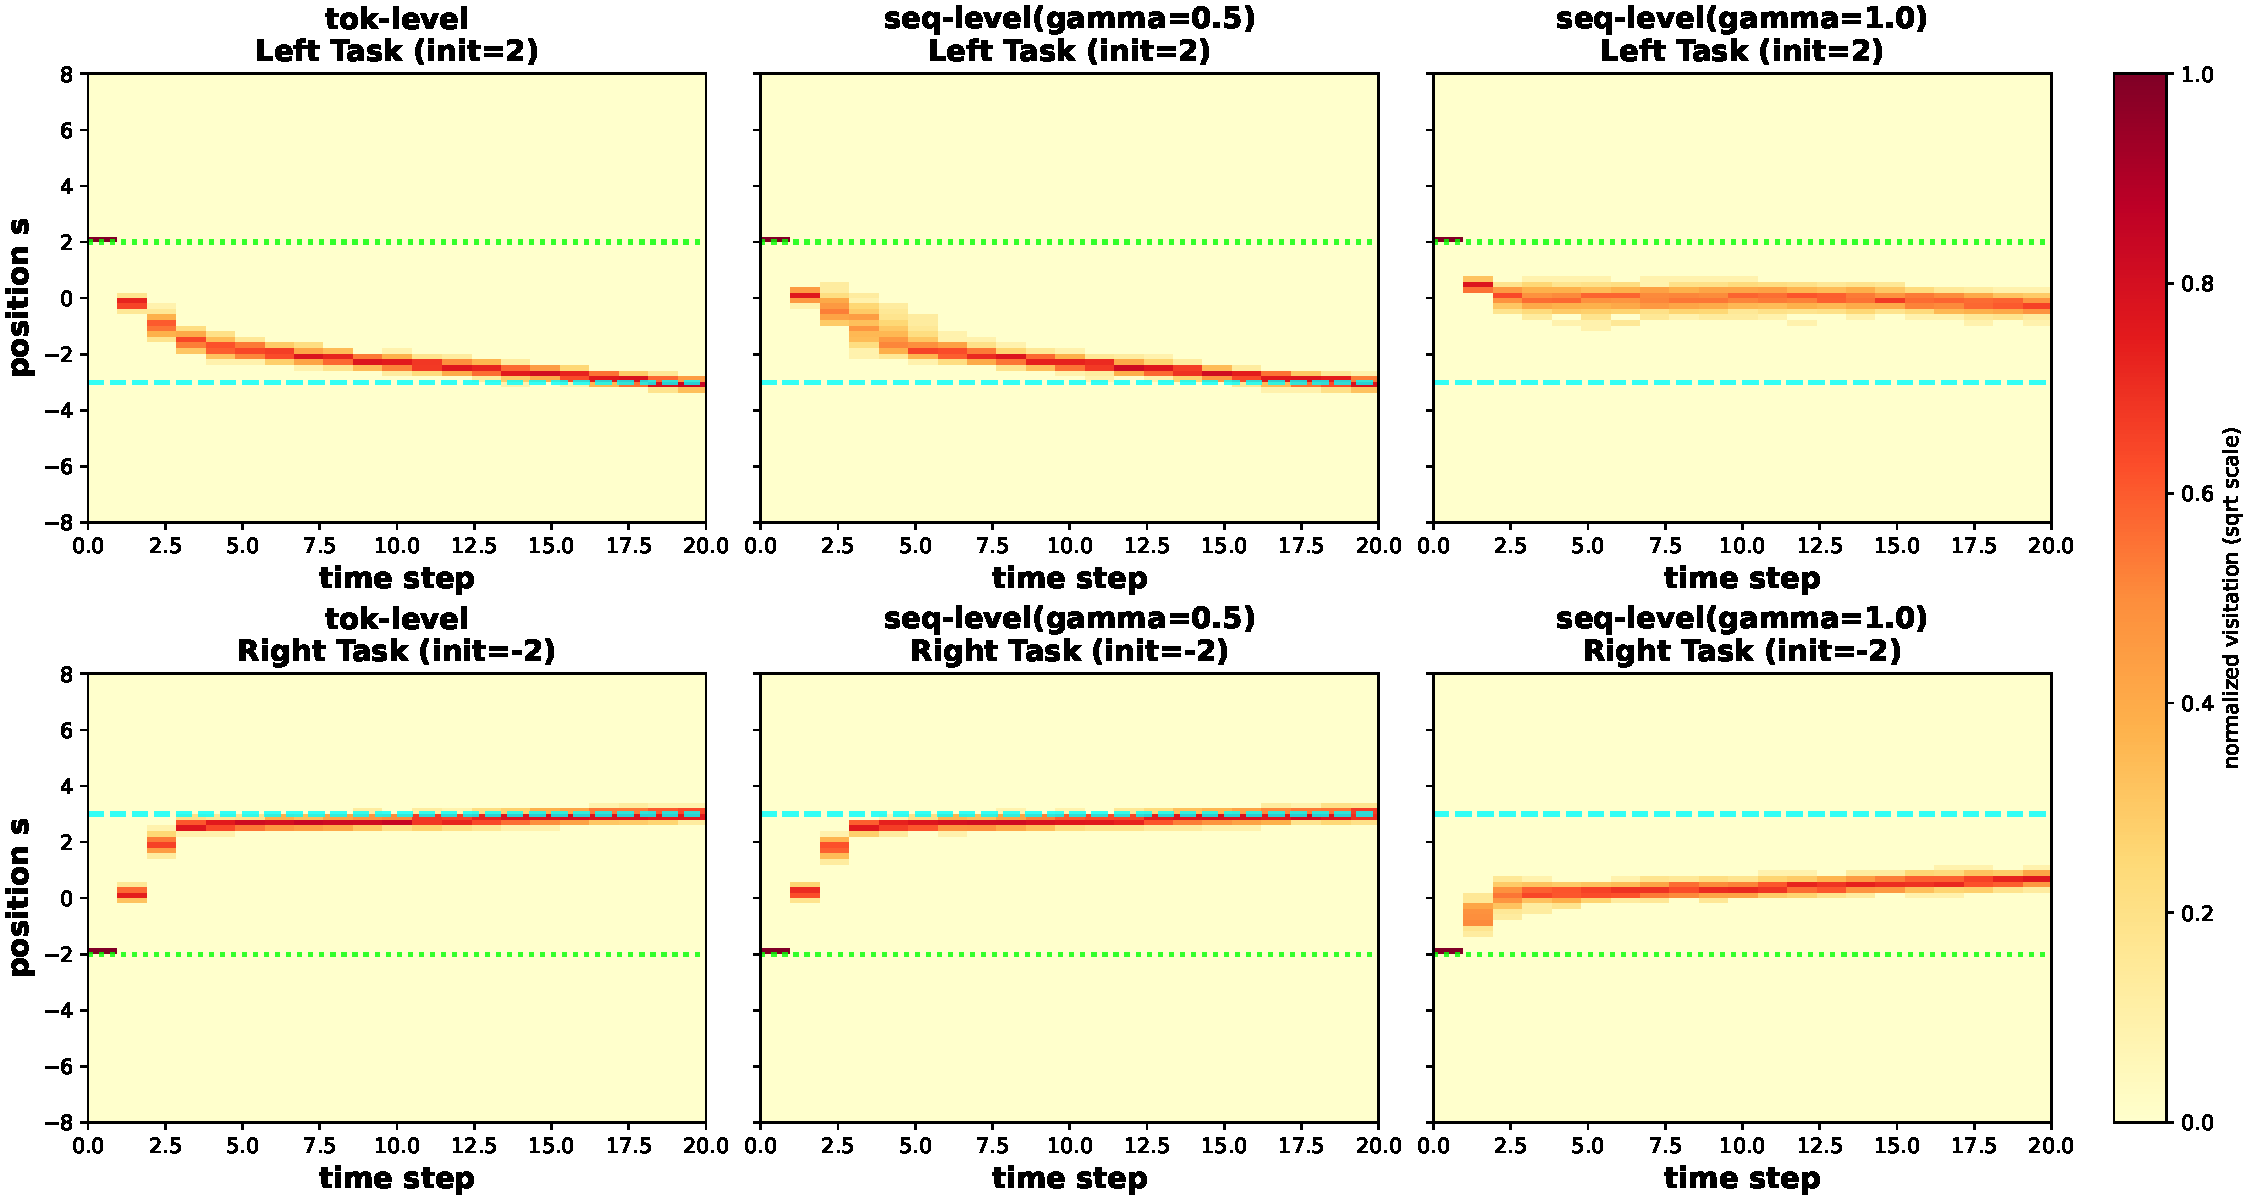
\includegraphics[width=\linewidth,height=4cm,keepaspectratio]{references/Revisiting On-Policy Distillation Empirical Failure Modes and Simple Fixes/figures/toy_heatmap42.pdf}
    \end{column}
  \end{columns}

  \vspace{0.1cm}
  \textbf{实验结果}：序列级OPD方差高出数个数量级且策略严重漂移；$\gamma \in \{0.0, 0.5\}$ 方差最低且稳定收敛。

  \vspace{0.1cm}
  \textbf{设计原则}：为了在长序列微调中控制梯度方差，应保持 token-level 的局部监督。
\end{frame}

% Slide 19: 问题 1.1
\begin{frame}[t]{\underline{问题2：}Sampled-Token的惩罚失衡}
  \begin{columns}[T,onlytextwidth]
    \begin{column}{0.48\textwidth}
      \begin{itemize}
        \item 在传统的 sampled-token OPD 中，每个位置的更新完全由单个采样 token 的对数比率驱动：$\log q(y_t \mid c_t) - \log \pi_\theta(y_t \mid c_t)$
        \item \textbf{惩罚倾斜}：如右图所示，绝大多数采样得到的 token 都收到了负奖励（即学生概率高于教师）。
        \item 优化易被极少数局部的正奖励 token 统治，导致模型对局部的过渡词、填充词非常敏感。
      \end{itemize}
    \end{column}
    \begin{column}{0.48\textwidth}
      \centering
      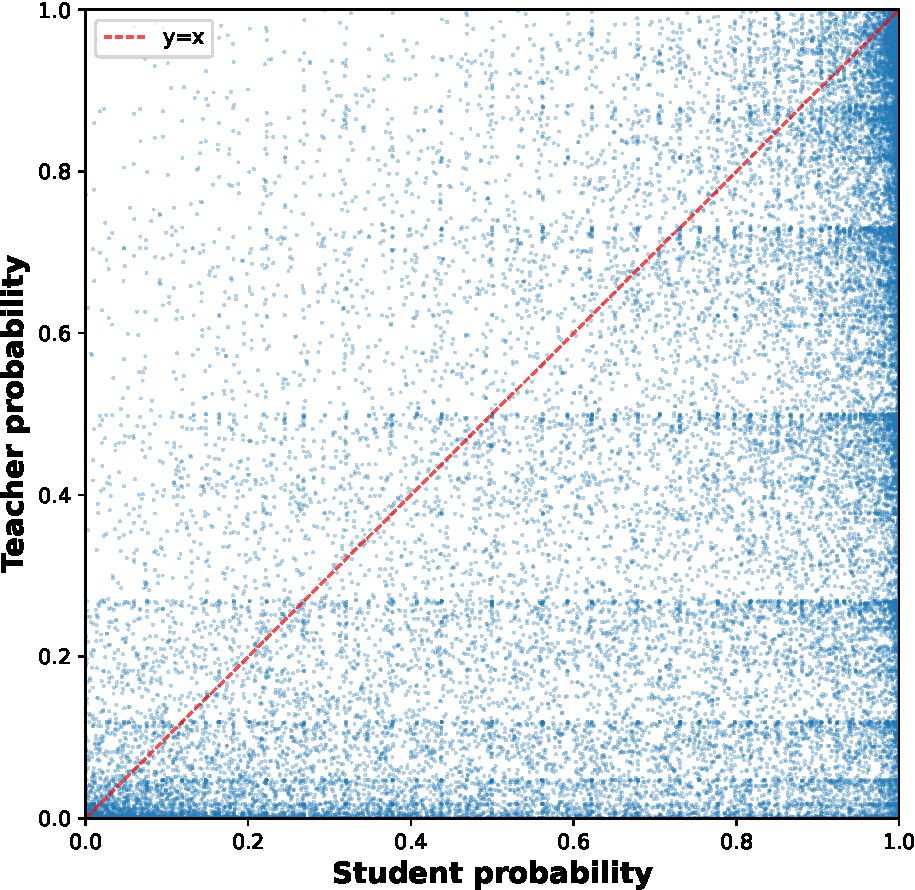
\includegraphics[width=\linewidth,height=4.2cm,keepaspectratio]{references/Revisiting On-Policy Distillation Empirical Failure Modes and Simple Fixes/figures/reward_scatter.pdf}
      \par\vspace{0.1cm}
      \footnotesize 首轮迭代师生 Token 概率散点图
    \end{column}
  \end{columns}
\end{frame}

% Slide 20: 问题 1.2
\begin{frame}[t]{\underline{问题3：}Tokenizer 与特殊 Token 不兼容}
  \begin{columns}[T,onlytextwidth]
    \begin{column}{0.38\textwidth}
      \begin{itemize}
        \item 师生分词器不同会导致相同文本的切分差异。
        \item \textbf{案例}：学生将 \texttt{<think>} 拆为 \texttt{<}、\texttt{think}、\texttt{>}，而教师期望 \texttt{<th}、\texttt{ink}、\texttt{>}。
      \end{itemize}
    \end{column}
    \begin{column}{0.6\textwidth}
      \centering
      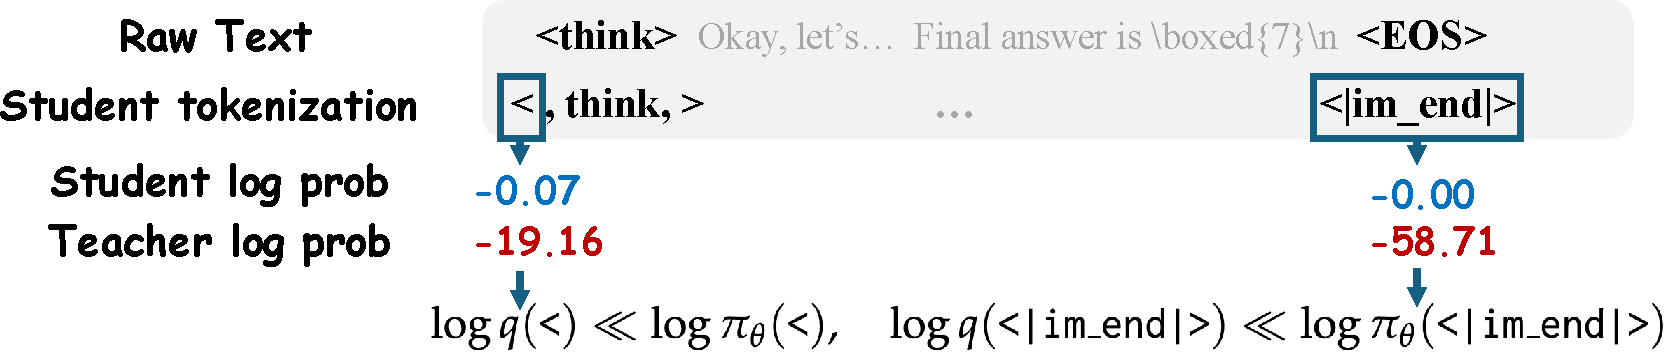
\includegraphics[width=\linewidth,height=3.6cm,keepaspectratio]{references/Revisiting On-Policy Distillation Empirical Failure Modes and Simple Fixes/figures/mismatch.pdf}
      \par\vspace{0.1cm}
      \footnotesize 师生 Tokenizer 冲突时的概率分布对比示例
    \end{column}
  \end{columns}
  \begin{itemize}
    \item 此时学生生成的 \texttt{<} 即使语义正确，也会在教师端收到极低概率，导致误罚。
  \end{itemize}
\end{frame}

% Slide 21: 现象 2.1
\begin{frame}[t]{\underline{问题4：}前缀漂移与教师指导失效}
  \begin{columns}[T,onlytextwidth]
    \begin{column}{0.32\textwidth}
      \textbf{局部对齐陷阱}：
      \begin{itemize}
        \item 当学生生成的轨迹发生偏移时，教师在学生前缀上的局部概率评估可能变得不合理。
        \item \textbf{案例}：学生陷入重复循环，但教师在重复 token 上的局部概率依然很高。
      \end{itemize}
    \end{column}
    \begin{column}{0.66\textwidth}
      \centering
      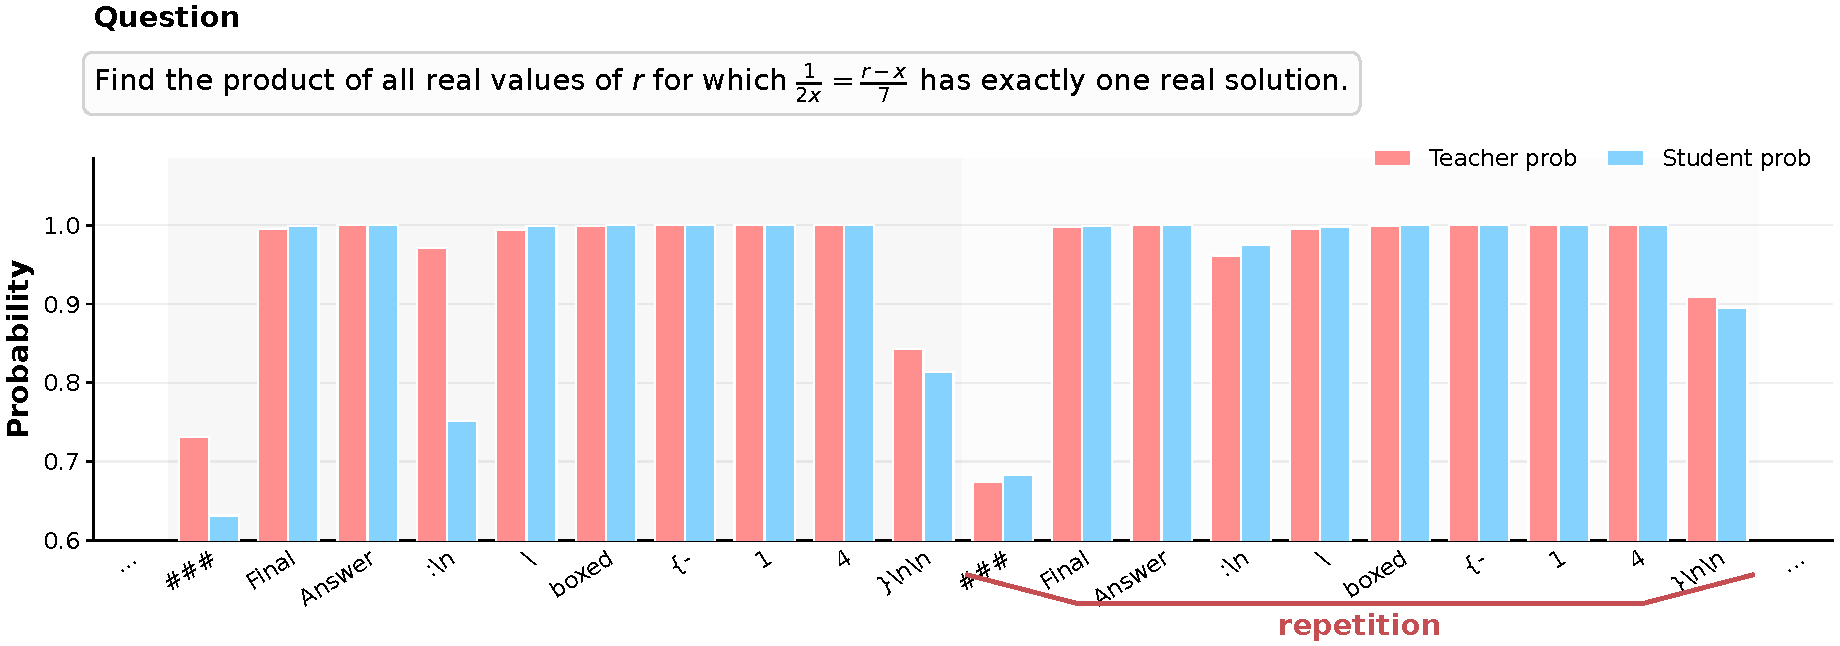
\includegraphics[width=\linewidth,height=4.2cm,keepaspectratio]{references/Revisiting On-Policy Distillation Empirical Failure Modes and Simple Fixes/figures/case/case_0_cropped.pdf}
      \par\vspace{0.1cm}
      \footnotesize 重复循环前缀下教师的局部高概率响应示例
    \end{column}
  \end{columns}
  \begin{itemize}
    \item 导致 sampled-token OPD 无法惩罚此类全局退化行为。
  \end{itemize}
\end{frame}

% Slide 22: 现象 2.2
\begin{frame}[t]{\underline{问题5：}随长度增加的信号衰减}
  \begin{columns}[T,onlytextwidth]
    \begin{column}{0.48\textwidth}
      \begin{itemize}
        \item 随着 rollout 生成长度增加，学生和教师策略的累积散度越严重。
        \item 如右图，随着 Token 位置后移，师生 log-probability 的差异分布明显展宽。
        \item 教师给出的单点指导信号在长生成路径的后半段变得高度嘈杂。
      \end{itemize}
    \end{column}
    \begin{column}{0.48\textwidth}
      \centering
      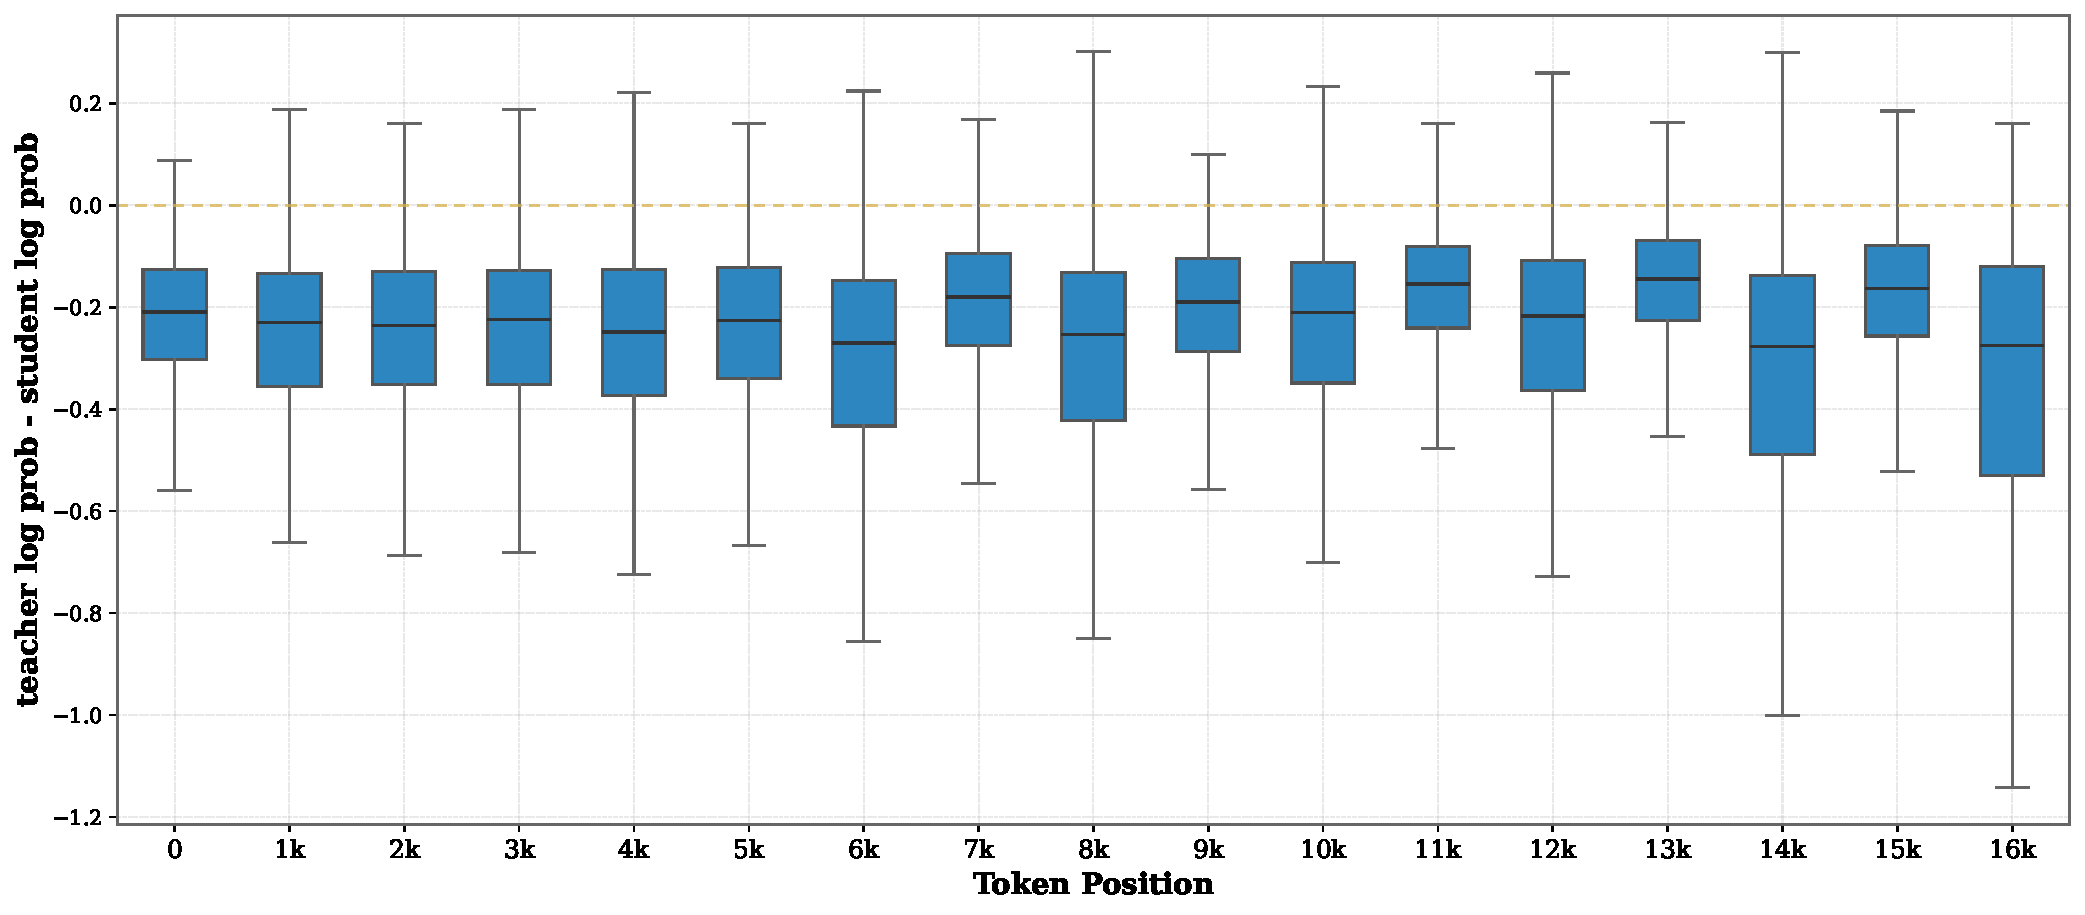
\includegraphics[width=\linewidth,height=4.0cm,keepaspectratio]{references/Revisiting On-Policy Distillation Empirical Failure Modes and Simple Fixes/figures/probgap_by_position.pdf}
      \par\vspace{0.1cm}
      \footnotesize 不同 token 位置下师生对数概率差的分布变化
    \end{column}
  \end{columns}
\end{frame}

% Slide 23: 方法 (1)
\begin{frame}[t]{核心方法：教师 Top-K 局部支持域匹配}
  \small
  \textbf{主要思想}：将单点 Token 采样对比，升级为在教师 top-$K$ 局部候选集上的分布匹配。
  
  \vspace{0.1cm}
  设教师 top-$K$ 支持集为 $S(c_t) \triangleq \mathrm{TopK}_q(c_t)$。在该支持集内重新归一化师生概率分布：
  \[
    \hat{\pi}_\theta(v \mid c_t) = \frac{\pi_\theta(v \mid c_t)}{\sum_{u \in S(c_t)}\pi_\theta(u \mid c_t)}, \qquad \hat{q}(v \mid c_t) = \frac{q(v \mid c_t)}{\sum_{u \in S(c_t)}q(u \mid c_t)}
  \]
  \textbf{局部支持域匹配 (Local Support Matching, LSM) 目标函数}：
  \[
    \mathcal{L}_{\mathrm{LSM}} = \mathbb{E}_{x,\, \{o_i\} \sim \pi_{\theta,\mathrm{infer}}} \left[ \frac{1}{\sum_{i=1}^{G} |o_i|} \sum_{i=1}^{G} \sum_{t=1}^{|o_i|} \sum_{v \in S(c_{i,t})} \hat \pi_\theta(v \mid c_{i,t}) \log \frac{\hat \pi_\theta(v \mid c_{i,t})}{\hat q(v \mid c_{i,t})} \right]
  \]
  \begin{itemize}
    \item 避免了单 sample log-ratio 的极高方差，使梯度由多高质量候选 Token 决定。
    \item 相比全词表对齐，仅在 top-$K$ 局部进行更新，计算开销极其低廉。
  \end{itemize}
\end{frame}

% Slide 24: 方法 (2)
\begin{frame}[t]{辅助方法：配套稳定化设计}
  \small
  为了保证 LSM 的训练稳定性，提出了以下三个关键的配套策略：
  
  \vspace{0.2cm}
  \textbf{1. 支持集重归一化 (Support Renormalization)}
  \begin{itemize}
    \item 仅在 top-$K$ 内部执行 softmax 归一化。
    \item 梯度不会泄露到支持集外部，使得师生局部概率质量具有可比性，防止训练崩溃。
  \end{itemize}
  
  \vspace{0.15cm}
  \textbf{2. Top-p Rollout 采样 (Top-$p$ Rollout Sampling)}
  \begin{itemize}
    \item 限制生成轨迹进入极端低频或胡言乱语的区域。
    \item 使学生生成的 prefix 保持在教师典型支持域内，从而使监督更具意义。
  \end{itemize}
  
  \vspace{0.15cm}
  \textbf{3. 特殊 Token 掩码 (Special-token Masking)}
  \begin{itemize}
    \item 排除 `<think>`、`<pad>` 等可能存在 tokenizer 差异的特殊 token，减少格式假阴性判罚。
  \end{itemize}
\end{frame}

% Slide 25: 实验结果 (1a) - 单任务数学推理指标对比
\begin{frame}[t]{\underline{实验结果：}单任务数学推理 (指标对比)}
  \textbf{评测设置}：学生 Qwen2.5-7B-Instruct，教师 OpenThinker3-7B。
  
  \vspace{0.15cm}
  \centering
  \small
  \begin{tabular}{lcccccc}
    \toprule
    \textbf{方法} & \textbf{Math500} & \textbf{AIME24} & \textbf{AIME25} & \textbf{Minerva} & \textbf{Olympiad} & \textbf{Avg.} \\
    \midrule
    Qwen2.5-7B-It & 68.2 & 13.3 & 0.0 & 26.5 & 32.9 & 28.2 \\
    OpenThinker3-7B & 92.2 & 53.3 & 40.0 & 39.0 & 55.6 & 56.0 \\
    \midrule
    Sampled-token OPD & 80.0 & 10.0 & 16.7 & 32.4 & 43.1 & 36.4 \\
    Sampled-token w/ mask & 81.4 & 26.7 & 16.7 & 34.2 & 44.7 & 40.7 \\
    \textbf{Ours w/o mask (LSM)} & 80.4 & 23.3 & \textbf{26.7} & 34.2 & 43.9 & \textbf{41.7} \\
    \textbf{Ours w/ mask (LSM)} & \textbf{82.0} & 23.3 & 23.3 & \textbf{34.9} & 43.9 & 41.5 \\
    \bottomrule
  \end{tabular}
  
  \vspace{0.2cm}
  \flushleft
  \begin{itemize}
    \item LSM 相比标准 OPD 在数学平均准确率上取得显著提升（+5.3\%）；
    \item LSM 在不使用特殊 token 掩码时依然取得最佳平均表现，表明其本身对 tokenizer 分词冲突极具韧性。
  \end{itemize}
\end{frame}

% Slide 26: 实验结果 (1b) - 单任务数学推理训练曲线
\begin{frame}[t]{\underline{实验结果：}单任务数学推理 (训练曲线)}
  \begin{itemize}
    \item LSM 在训练过程中准确率稳步上升，未出现由于高方差导致的突然退化。
    \item top-$K$ 局部对齐提供了更加平滑的优化路径。
  \end{itemize}

  \vspace{0.1cm}
  \centering
  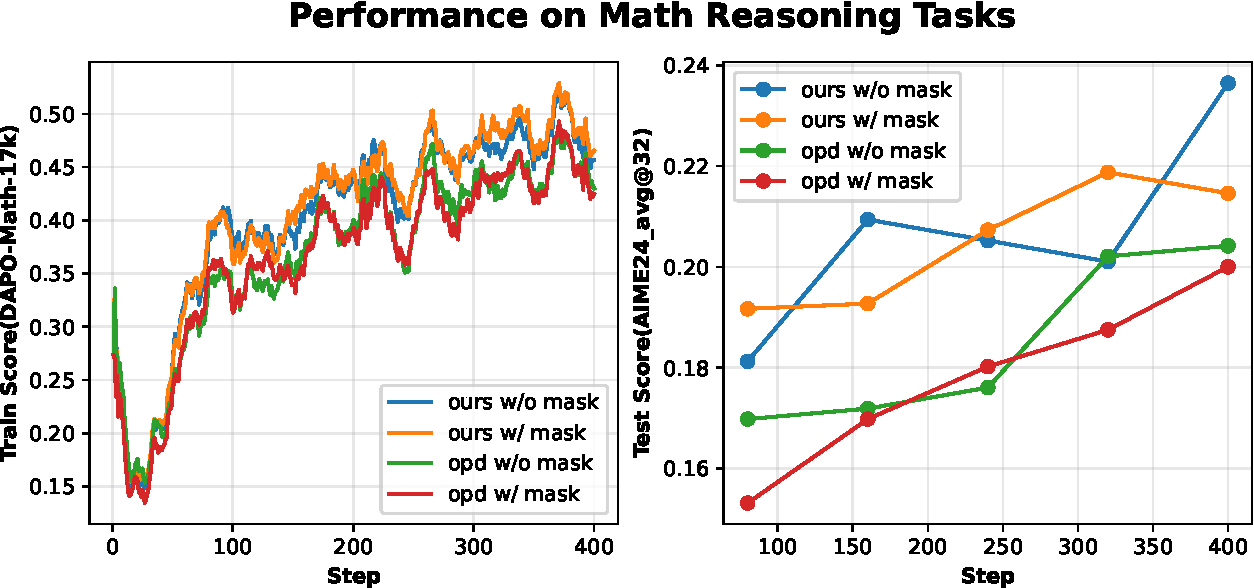
\includegraphics[width=0.75\linewidth,height=5cm,keepaspectratio]{references/Revisiting On-Policy Distillation Empirical Failure Modes and Simple Fixes/figures/curves_single_task.pdf}
  \par\vspace{0.05cm}
  \footnotesize 单任务数学训练下的测试准确率收敛曲线
\end{frame}

% Slide 27: 实验结果 (2a) - 多任务对齐训练指标对比
\begin{frame}[t]{\underline{实验结果：}多任务对齐训练 (指标对比)}
  \textbf{混合设置}：数学教师 OpenThinker3-7B，Agent (ALFWorld) 教师 GiGPO-Qwen2.5-7B-It。
  
  \vspace{0.15cm}
  \centering
  \small
  \begin{tabular}{lcccccc}
    \toprule
    \textbf{方法} & \textbf{ALFWorld} & \textbf{MATH500} & \textbf{AIME24} & \textbf{Minerva} & \textbf{Olympiad} & \textbf{Math Avg.} \\
    \midrule
    Qwen2.5-7B-It & 21.9 & 68.2 & 13.3 & 26.5 & 32.9 & 28.2 \\
    \midrule
    Sampled-token OPD & 90.6 & 74.8 & 13.3 & 32.1 & 40.5 & 34.8 \\
    Sampled-token w/ mask & 93.8 & 76.0 & 20.0 & 33.5 & 40.4 & 36.6 \\
    \textbf{Ours w/o mask (LSM)} & 95.3 & \textbf{82.0} & \textbf{33.3} & 32.7 & \textbf{44.0} & \textbf{41.7} \\
    \textbf{Ours w/ mask (LSM)} & \textbf{97.7} & 79.0 & 20.0 & \textbf{34.6} & 42.5 & 38.6 \\
    \bottomrule
  \end{tabular}
  
  \vspace{0.2cm}
  \flushleft
  \begin{itemize}
    \item LSM 显著提升了数学的跨任务泛化（Math Avg 从 34.8\% 提高到 \textbf{41.7\%}）；
    \item 在 Agent 任务（ALFWorld）上，LSM 配合掩码也取得了最佳对齐成功率 (\textbf{97.7\%})。
  \end{itemize}
\end{frame}

% Slide 28: 实验结果 (2b) - 多任务对齐训练曲线
\begin{frame}[t]{\underline{实验结果：}多任务对齐训练 (收敛曲线)}
  \begin{itemize}
    \item 在多任务混合对齐中，LSM 表现出了显著好于标准 OPD 的学习效率。
    \item 能够在保持或提升 Agent 能力的同时，快速拉升数学的推理精度。
  \end{itemize}

  \vspace{0.1cm}
  \centering
  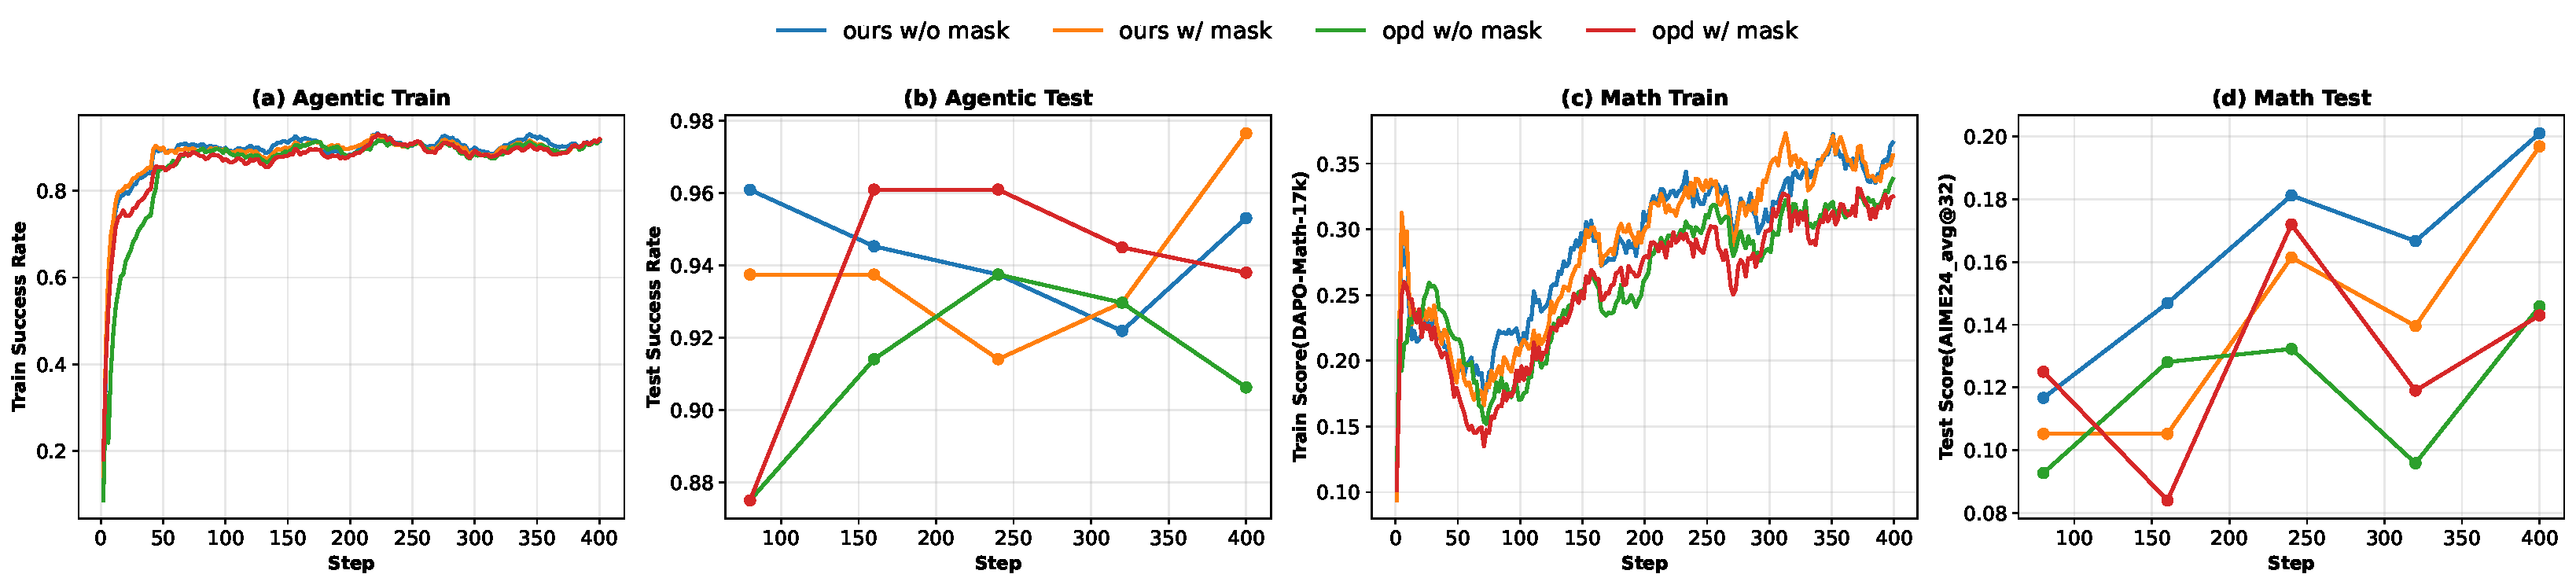
\includegraphics[width=0.95\linewidth,height=5cm,keepaspectratio]{references/Revisiting On-Policy Distillation Empirical Failure Modes and Simple Fixes/figures/curves_multi_task.pdf}
  \par\vspace{0.05cm}
  \footnotesize 多任务对齐训练下的数学准确率收敛曲线
\end{frame}

% Slide 33: 总结
\begin{frame}[t]{总结}
  \begin{columns}[T,onlytextwidth]
    \begin{column}{0.48\textwidth}
      \textbf{Sampled-Token OPD 的五个痛点}
      \begin{itemize}
        \item 序列级方差随长度 $T^4$ 增长，被迫使用 token-level 局部更新；
        \item 单 token 采样导致严重惩罚倾斜（多数 token 收到负奖励）；
        \item 师生分词器不兼容导致格式 token 误罚；
        \item 前缀漂移使教师在偏离轨迹上给出误导性高概率；
        \item 随生成长度增加，师生分布发散导致信号衰减。
      \end{itemize}
    \end{column}
    \begin{column}{0.48\textwidth}
      \textbf{LSM 提供的最佳 Recipe}
      \begin{itemize}
        \item \textbf{Teacher top-$K$ 局部支持域匹配}：在 top-$K$ 支持域内进行分布级别的对齐，极低代价提供稳定的监督。
        \item 支持集 Renormalization：防梯度泄露，不可或缺。
        \item Top-$p$ 采样：规范 rollout，降低前缀漂移速度。
        \item 特殊 Token 掩码：隔绝分词器格式冲突带来的干扰。
      \end{itemize}
    \end{column}
  \end{columns}
\end{frame}

\section{References}
\begin{frame}[allowframebreaks]{参考文献}
  \footnotesize
  \begin{thebibliography}{9}
    \bibitem{rethinking} Yaxuan Li, Yuxin Zuo, Bingxiang He, Jinqian Zhang, Chaojun Xiao, Cheng Qian, Tianyu Yu, Huan-ang Gao, Wenkai Yang, Zhiyuan Liu, Ning Ding. \textit{Rethinking On-Policy Distillation of Large Language Models: Phenomenology, Mechanism, and Recipe}. arXiv:2604.13016, 2026.
    \bibitem{revisiting} Yuqian Fu, Haohuan Huang, Kaiwen Jiang, Jiacai Liu, Zhuo Jiang, Yuanheng Zhu, Dongbin Zhao. \textit{Revisiting On-Policy Distillation: Empirical Failure Modes and Simple Fixes}. arXiv:2603.25562, 2026.
  \end{thebibliography}
\end{frame}

\end{document}
